% --------------------------------------------------------------
% This is all preamble stuff that you don't have to worry about.
% Head down to where it says "Start here"
% --------------------------------------------------------------

\documentclass[12pt]{article}

\usepackage[margin=1in]{geometry} 
\usepackage{amsmath,amsthm,amssymb}
\usepackage{graphicx}
\usepackage{float}
\usepackage{bm}
\usepackage{hyperref}

\newcommand{\N}{\mathbb{N}}
\newcommand{\Z}{\mathbb{Z}}


\begin{document}
	
	% --------------------------------------------------------------
	%                         Start here
	% --------------------------------------------------------------
	
	%\renewcommand{\qedsymbol}{\filledbox}
	
	\title{Notes on Object Detection}%replace X with the appropriate number
	\author{Tim Hsu} %if necessary, replace with your course title
	\date{}
	\maketitle
	
	\section*{Task}
	Object detection is the combination of the tasks of localization and classification, i.e. the task of locating salient objects in an image. Given an image, object detection seeks to return a set of bounding boxes of each object in the image and a prediction of the class of the object contained in each box.
	
	\section*{Metrics}
	\subsection*{mAP: Mean Average Precision}
	\[precision = \frac{TP}{TP+FP}=\frac{TP}{\textrm{all positive predictions}}\]
	\[recall = \frac{TP}{TP+FN}=\frac{TP}{\textrm{all positive ground truths}}\]
	\[IoU = \frac{\textrm{overlapping area}}{\textrm{union area}}\]
	
	In the context of object detection, a prediction is usually considered to be correct if $IoU > 0.5$. The average precision is the average of maximum precision at 11 recall levels: $\{0, 0.1, 0.2,...,0.9, 1.0\}$:
	\[AP = \frac{1}{11}\left(AP_r(0)+AP_r(0.1)+AP_r(0.2)+...+AP_r(0.9)+AP_r(1.0)\right)\]
	
	Example: we have an image with 5 objects. We sort our predictons based on the confidence levels and take the top-$k$ predictions. For each $k$, we get a different $precision$ and $recall$. For example, let's say we take the top-4 predictions, and 3 of them are correct. Our $precision$ and $recall$ are thus:
	\[precision = \frac{3}{4}=0.75\]
	\[recall = \frac{3}{5} = 0.6\]
	Repeat this for each rank until we hit $recall=1.0$, we get the following table.
	\begin{center}
			\begin{tabular}{|c|c|c|}
			\hline
			Rank & Precision & Recall\\\hline
			1 & 1.0 & 0.2\\            \hline
			2 & 1.0 & 0.4\\            \hline
			3 & 0.66 & 0.4\\           \hline
			\textbf{4} & \textbf{0.75} & \textbf{0.6}\\           \hline
			5 & 0.6 & 0.6\\            \hline
			6 & 0.66 & 0.8\\           \hline
			7 & 0.57 & 0.8\\           \hline
			8 & 0.5 & 0.8\\            \hline
			9 & 0.44 & 0.8\\           \hline
			10 & 0.5 & 1.0\\          
			\hline
		\end{tabular} 
	\end{center}

	$AP_r(0.6)$ is the maximum of the precision at ranks where $recall \ge 0.6$, i.e.
	\[AP_r(0.6) = \max(0.75, 0.6, 0.66, 0.57, 0.5, 0.44, 0.5)=0.75\]
	
	Taking the average of that on all 10 recall levels, we obtain the $AP$. Taking the average of $AP$ for all obejct classes, we obtain the $mAP$.\\
	
	In recent research papers, people tend to generate $mAP$ metric for different $IoU$ levels. For example, on the MS-COCO dataset, people usually report $\mathbf{mAP@[0.5:0.95]}$, which denotes the average $mAP$ for $IoU$ from 0.5 to 0.95, with step size of 0.05.
	
	
	\section*{Challenges}
	\begin{itemize}
		\item variable number of objects: an image can consists of any amount of objects
		\item resizing: an object can be of any size. Moreover, objects in a single image may likely have very different sizes from another object in the same image.
	\end{itemize}

	\section*{Approaches}
	\subsection*{OverFeat}
	Combines sliding-window method with CNN. Really slow.
	
	\subsection*{R-CNN}
	\begin{enumerate}
		\item Region proposal with selective search
		\item Extract features from each region with CNN
		\item Classify each region with SVM
	\end{enumerate}
	
	Multiple stages, not end-to-end
	
	\subsubsection*{Selective Search}
	\begin{enumerate}
		\item Segmentation to generate candidate objects
		\item Combine \textbf{similar} regions to larger ones
		\subitem * similarity using color, texture, size, shape, compatibility (how well two regions/shapes fit together)
		\item Use combined regions to generate candidate 
	\end{enumerate}
	
	\subsection*{Fast R-CNN}
	\begin{enumerate}
		\item Region proposal with selection search
		\item Region of Interest (RoI) pooling on image feature map
		\item Object classification and per-class bounding box regression
	\end{enumerate}

	\begin{itemize}
		\item use of anchors
	\end{itemize}

	\subsection*{Faster R-CNN}
	Three main modules:
	\begin{enumerate}
		\item RPN (Region Proposal Network)
		\item RoIP (Region of Interest Pooling)
		\item Object classification and per-class bounding box regression
	\end{enumerate}

	\subsubsection*{RPN}
	Rather than using the Selective Search method like previous architectures, the Faster R-CNN architecture uses a Region Proposal Network, which takes an image as input and outputs a set of rectangular object proposals, each with a probability score of it being an object (object vs. background).
	
	We first use the intermediate layer of a CNN (usually pretrained on a image classification task) to map a raw image to a convolutional feature map.
	\begin{figure}[H]
		\centering
		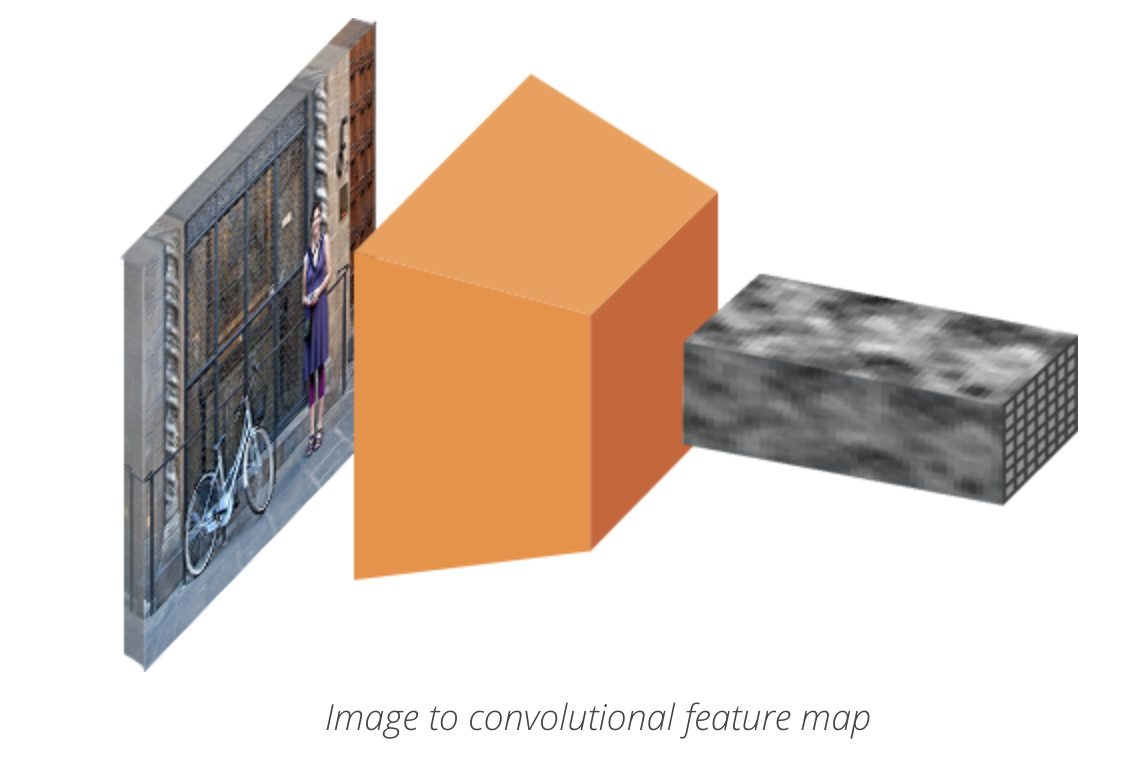
\includegraphics[width=0.5\linewidth]{figures/image-to-feature}
	\end{figure}
	To come up with proposals, the RPN uses \textbf{anchors}. Rather than simply predicting 8 numbers (2 coordinates for each of the 4 corners), the RPN structures a regression problem based on reference boxes. It takes a reference box with attributes $x_{center}, y_{center}, width, height$ and tries to predict 4 numbers $\Delta x_{center}, \Delta y_{center}, \Delta width, \Delta height$ that best modifies the reference box to fit objects.
	
	\textbf{Anchors} are the reference bounding boxes placed throughout the image that the RPN modifies to perform object detection. One thing to note is that these anchors are placed on the convolutional feature map, but the final anchors actually reference the original image. We create a set of anchors for each of the points in the convolutional feature map of dimension $conv_{width} \times conv_{height}$.
	
	\begin{figure}[H]
		\centering
		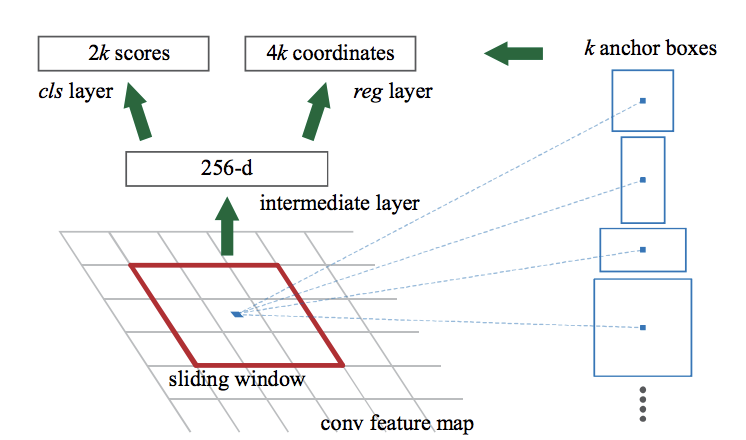
\includegraphics[width=0.5\linewidth]{figures/RPN}
	\end{figure}
	
	The RPN then slides over the convolutional feature map, taking a $n\times n$ window as the input. The input convolutional features are mapped to a lower dimensional feature. The feature is then fed to two fully connected layer, box-regression and box-classification, generating the box modification attributes and the objectness score, respectively. At each window location, the RPN predicts up to $k$ region proposals simultaneously. In the original paper, $k=9$, i.e. they set 9 anchors at each position, the combination of 3 scales and 3 ratios. There will be a total of $conv_{width}\times conv_{height} \times k$ anchors. This approach is translation-invariant, i.e. if an object is translated in an image, the proposal should translate as well.
	\\\\
	\textbf{Loss function}
	RPN is trained with a loss function that is the combination of the loss from the regression layer and the classification layer. RPNs assign a binary objectness label to each anchor in the following way:
	\begin{itemize}
		\item Positive label: (1) anchor with the highest IoU with a ground-truth box or (2) anchor that has an IoU higher than 0.7 with any ground-truth
		\item Negative label: anchor IoU is lower than 0.3 with all ground-truth boxes
	\end{itemize}
	Anchors that are neither positive nor negative do not contribute to training. The multi-task loss for an image is:
	\[L(\{p_i\},\{t_i\}) = \frac{1}{N_{cls}}\sum_{i}L_{cls}(p_i, p_i^*) + \lambda\frac{1}{N_{reg}}\sum_{i}p_i^*L_{reg}(t_i,t_i^*)\]
	where $p_i$ is the predicted probability of an anchor $i$ being an object, and $p*_i$ is 1 if an anchor is assigned a positive label, 0 otherwise. $L_{cls}$ is the log loss of objectness prediction. The classification loss is normalized by the size of the mini-batch.
	\\\\
	$t_i$ is the 4 parameterized coordinates of the predicted bounding box and $t_i^*$ is the parameterized coordinate of the associated ground-truth box with the anchor. The regression loss $L_reg(t_i, t_i^*)=R(t_i-t_i^*)$ is the smooth L1 loss function. Note that the regression loss is only activated for positive anchors. The regression term is normalized by the number of anchor locations on the images. The 4 coordinates are parameterized in the following way:
	\begin{eqnarray*}
		t_x &=& \frac{x-x_a}{w_a}\\
		t_y &=& \frac{y-y_a}{h_a}\\
		t_w &=& \log(\frac{w}{w_a})\\
		t_y &=& \log(\frac{h}{h_a})
	\end{eqnarray*}
	where $x, x_a, and x^*$ are the coordinate for the predicted box, anchor box, and ground-truth box, respectively.

	\subsubsection*{RoIP}
	Now that the RPN generated the proposals, we are left with a bunch of unclassified proposals, all of different sizes. Intuitively, we can classify each and every proposal, which often takes a lot of time. RoI pooling converts the features inside a valid region of interest into a small feature map of a fixed size $H\times W$. It divides the original $h\times w$ RoI window into a smaller $H\times W$ grid of sub-windows, each of size $h/H \times w/W$, and takes the max values of each sub-window. See animation at \url{https://deepsense.ai/wp-content/uploads/2017/02/roi_pooling-1.gif}
	
	\subsubsection*{R-CNN}
	Finally, a region-based CNN (R-CNN) is used to perform the image classification. In implementation, this network shares the convolutional feature weights with the RPN. On top of classification, another objective of the R-CNN is to adjust the bounding box according to the predicted class.\\
	\\
	The R-CNN takes the feature maps of each proposal and pass it through 2 linear layers. Then, it maps the outcome to two output layers:
	\begin{itemize}
		\item a linear layer with $N+1$ unis for the $N$ classes and 1 for background class
		\item a linear layer with $4N$ units for $\Delta x, \Delta y, \Delta w, \Delta h$ for each possible classes
	\end{itemize}

	\subsection*{Bottom-up and Top-bottom Attention Model for Image Captioning}
	This paper describes a  framework based on an object detection model and an image captioning model combined. The object detection model is optimized to generate bounding boxes and predict the attribute and class of the object in the bounding boxes. However, the prediction on attribute and class were not actually used in this approach.
	\\
	\\
	\begin{figure}[H]
		\centering
		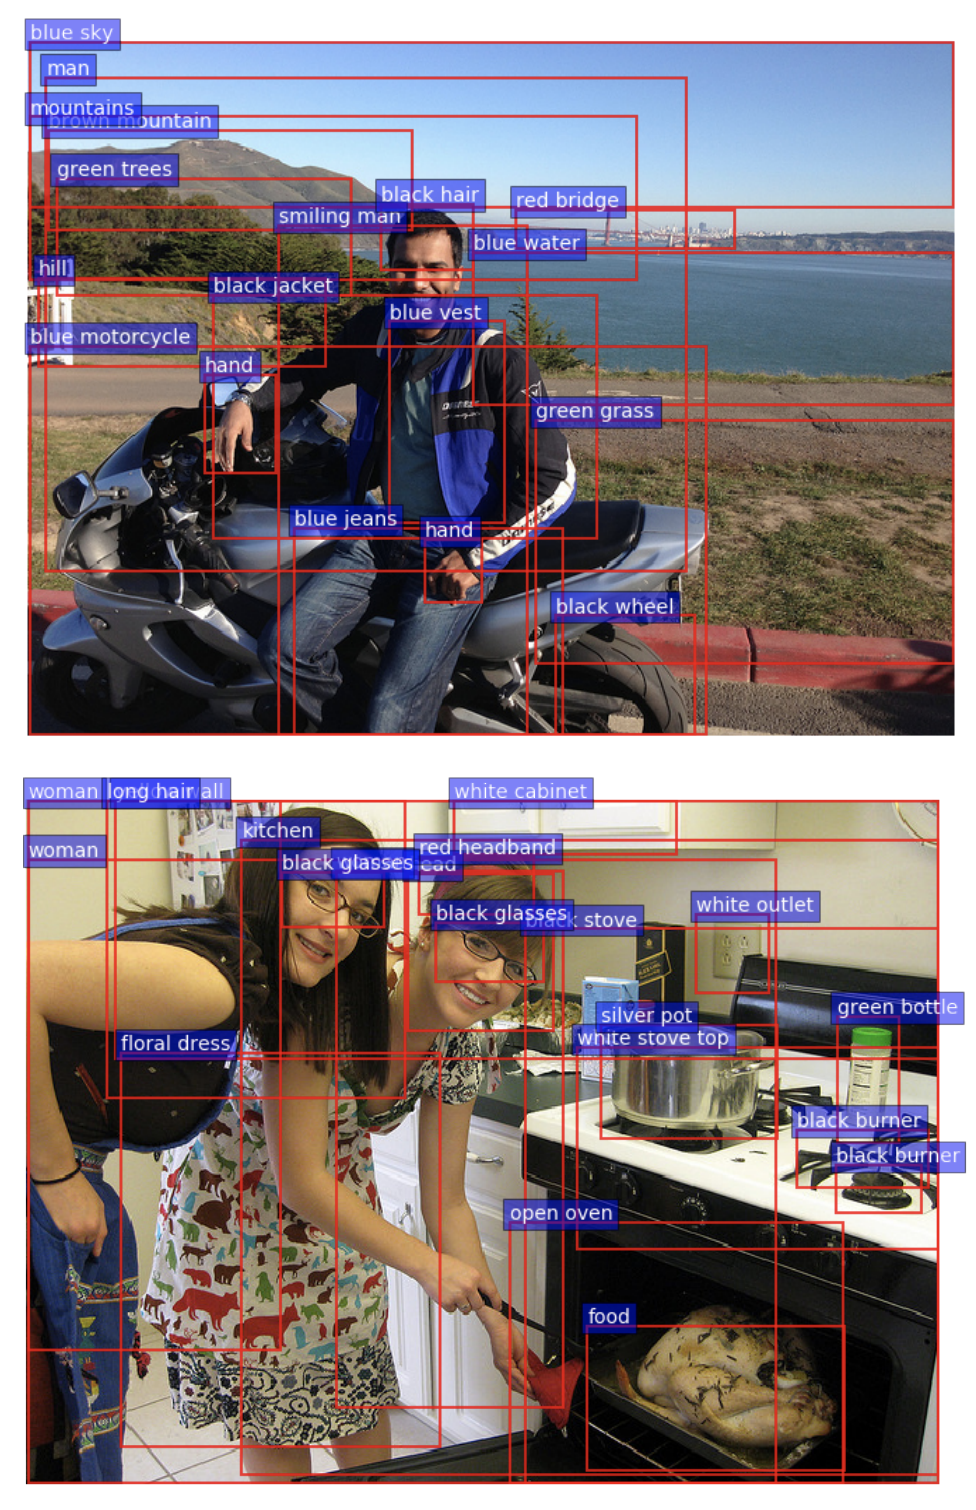
\includegraphics[width=0.5\linewidth]{figures/faster-rcnn-output}
	\end{figure}
	For a single image, the image captioning model takes in a variably-sized set of image features $V=\{\bm{v}_1, \bm{v}_2,...,\bm{v}_k\}, \bm{v}_i \in \mathbb{R}^{D}$. This set of image features is the output of the specified object detection model, which, in the context of this framework, is a Faster R-CNN model. Since only salient regions consisting object are outputted from the Faster R-CNN, this can be viewed as a ``hard-attention'' mechanism.\\
	\\
	\begin{figure}[H]
		\centering
		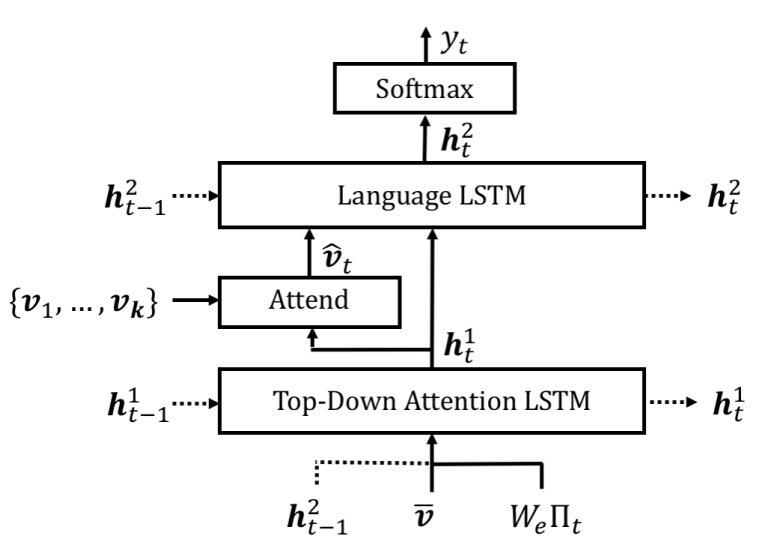
\includegraphics[width=0.5\linewidth]{figures/image-caption}
	\end{figure}
	The image captioning model itself consists of two components, described as two layers of LSTM: 1) top-down attention model with hidden states $h_t^1$ and 2) language model with hidden states $h_t^2$. \\
	\\
	The top-down attention LSTM aims to provide a properly attended image feature to the language model LSTM for better caption generation. It takes as input the concatenation of the previous hidden state $h_{t-1}^2$ of the language model, the mean-pooled image feature $\bar{v} = \frac{1}{k}\sum_{i}\mathbf{v}_i$, and the word embedding $W_e\left[w_t\right]$ of the previously generated word all concatenated together, i.e.:
	\[x_t = \left[h_{t-1}^2, \bm{\bar{v}}, W_e\left[w_t\right]\right]\]
	The normalized attention weight $\alpha_{i, t}$ for each of the $k$ image features $\mathbf{v}_i$ is:
	\begin{eqnarray*}
		a_{i, t} &=& w_a^T \tanh\left(W_{va}\bm{v}_i+W_{ha}h_t^1\right)\\
		\bm{\alpha}_{t} &=& \textrm{softmax}(\bm{a_t})
	\end{eqnarray*}
	The attended image feature $\hat{\bm{v}_t}$ is obtained by:
	\[\hat{\bm{v}_t} = \sum_{i} \alpha_{i, t} \bm{v}_t\]
	\noindent
	$\hat{\bm{v}}_t$ is then concatenated with $h_t^1$ as the input $\bm{x}_t^2$ to the second layer language LSTM:
	\[\bm{x}_t^2 = \left[\bm{\hat{\bm{v}_t}, h_t^1}\right],\]
	which then generates the output word by word at each timestep $t$ as a language model LSTM would by ouputting a vector $\bm{y}_t \in \mathbb{R}^{|\Sigma|}$ by
	\[\bm{y}_t = \textrm{softmax}(W_p\bm{h}_t^2 + \bm{b_p})\]
	Due to the bottom-up attention from the image features extracted from Faster R-CNN and the top-down attention in the image caption model, this approach takes into account both small detailed object in the image and large region objects. Furthermore, the model is able to simultaneously consider multiple objects that might be related in the image. This can be seen in the example below, where the region with maximum attention weights at each time step are outlined in red. The model is able to focus on the frisbee when generating the word `playing' and also attend to the large black region in the background when generating the words `black' and `field'.
	\begin{figure}[H]
		\centering
		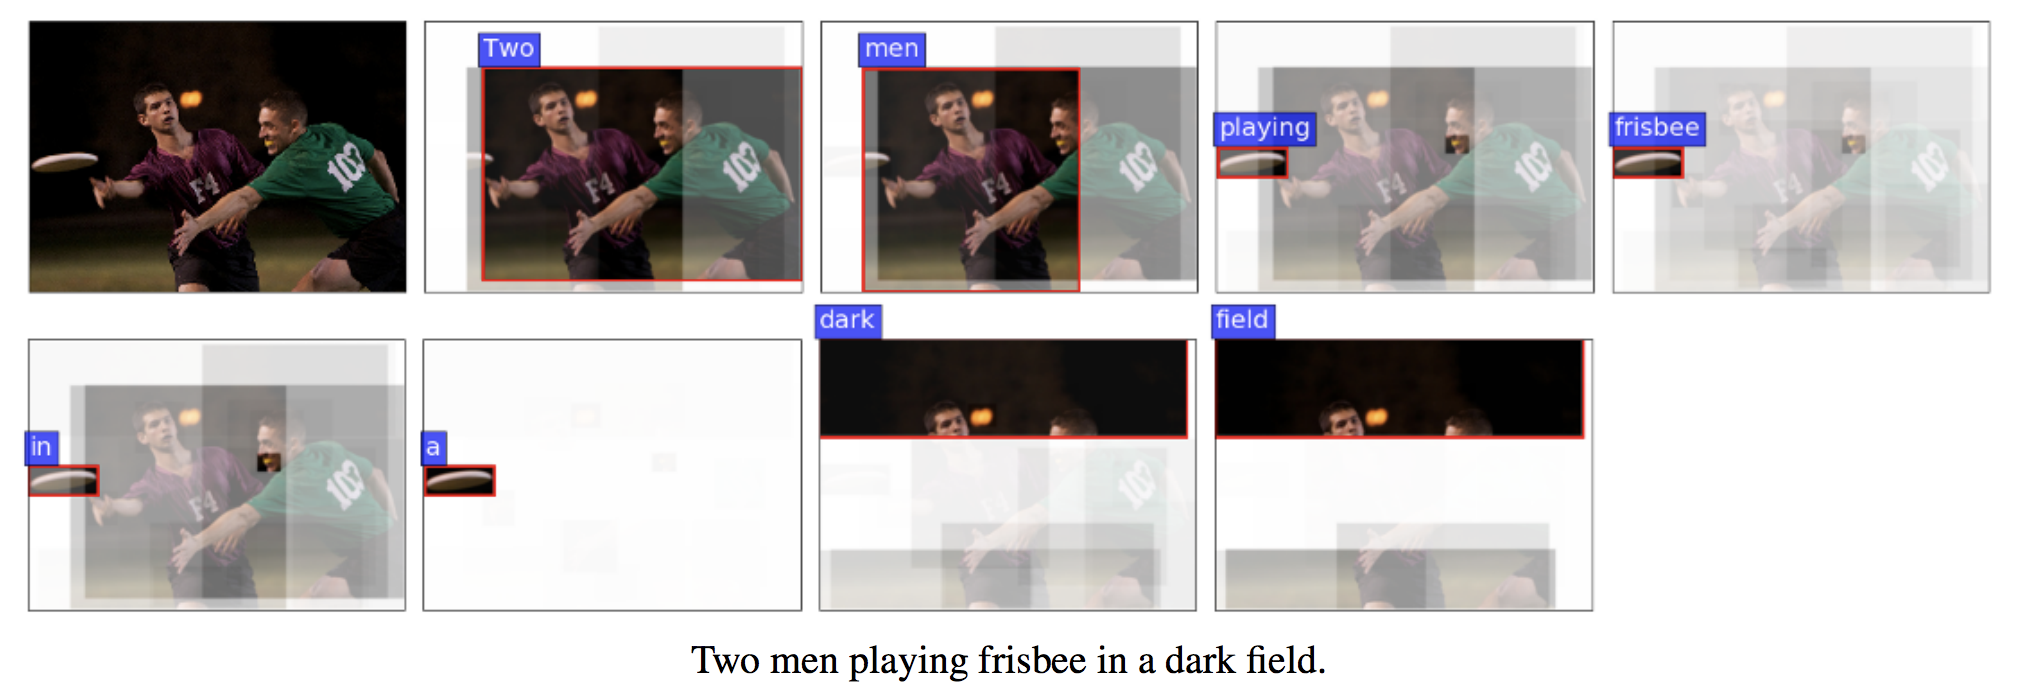
\includegraphics[width=\linewidth]{figures/attention-example}
	\end{figure}
	Examples of comparison between the method of show-and-tell (left) and this approach (right) by He Lu on the AI Challenger image caption dataset:
	\begin{figure}[H]
		\centering
		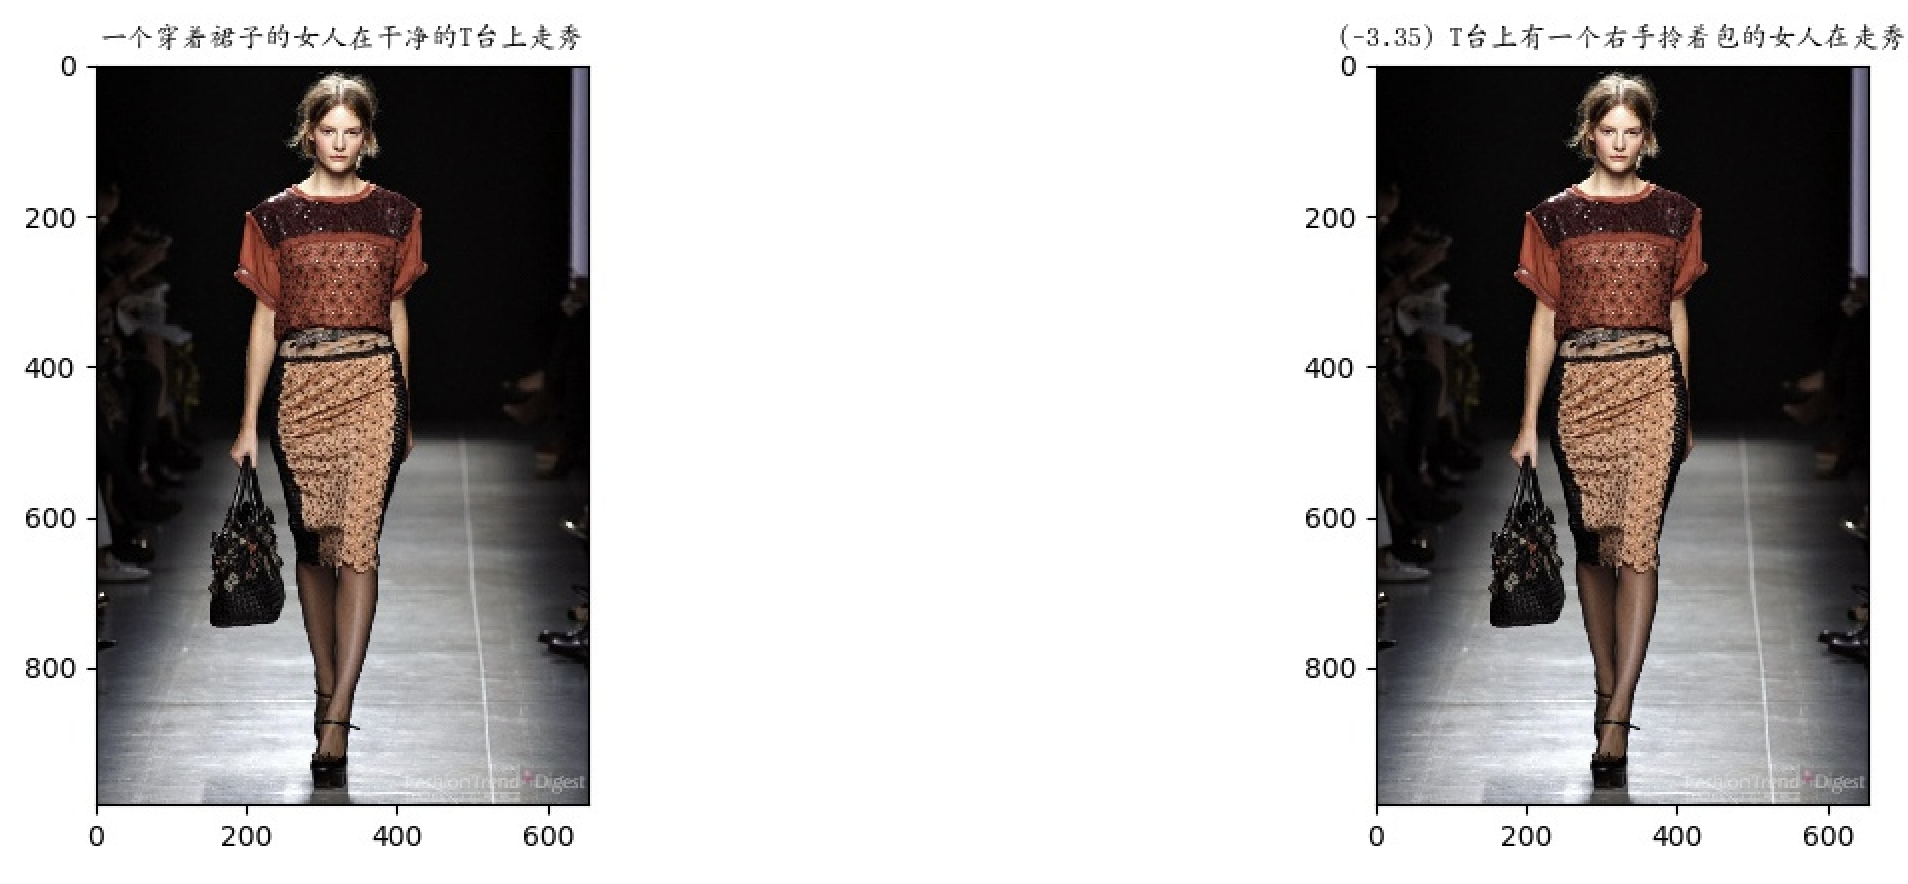
\includegraphics[width=\linewidth]{figures/comparison-1}
	\end{figure}
	\begin{figure}[H]
		\centering
		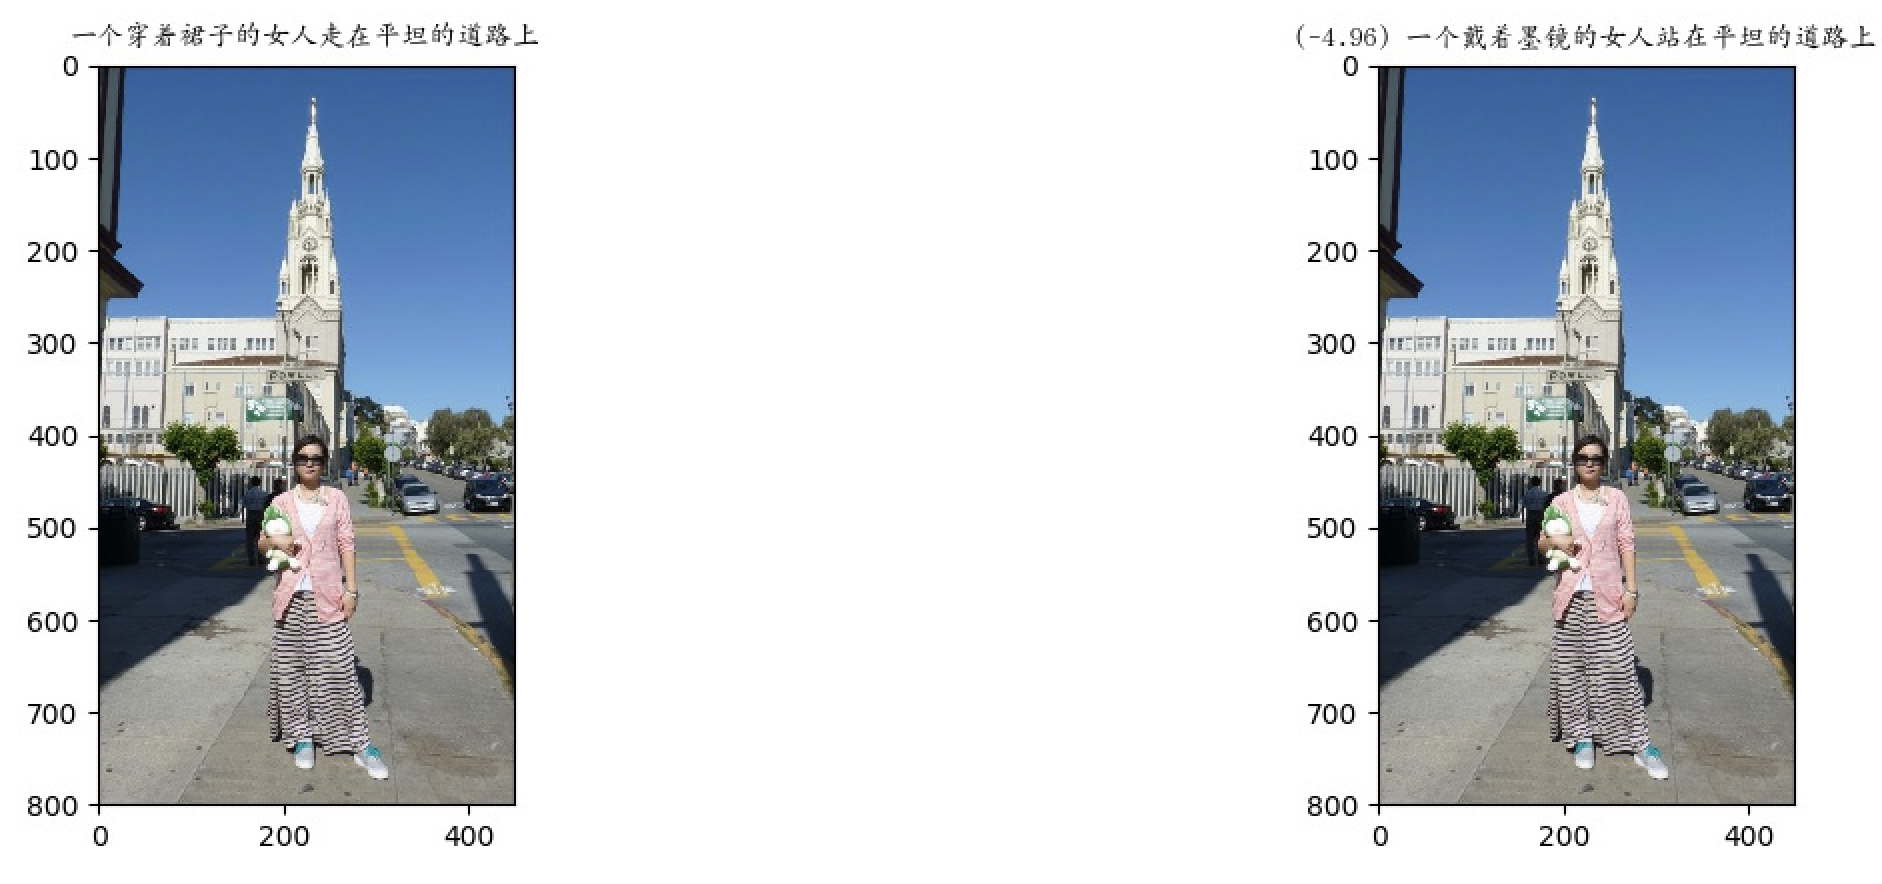
\includegraphics[width=\linewidth]{figures/comparison-2}
	\end{figure}
	\begin{figure}[H]
		\centering
		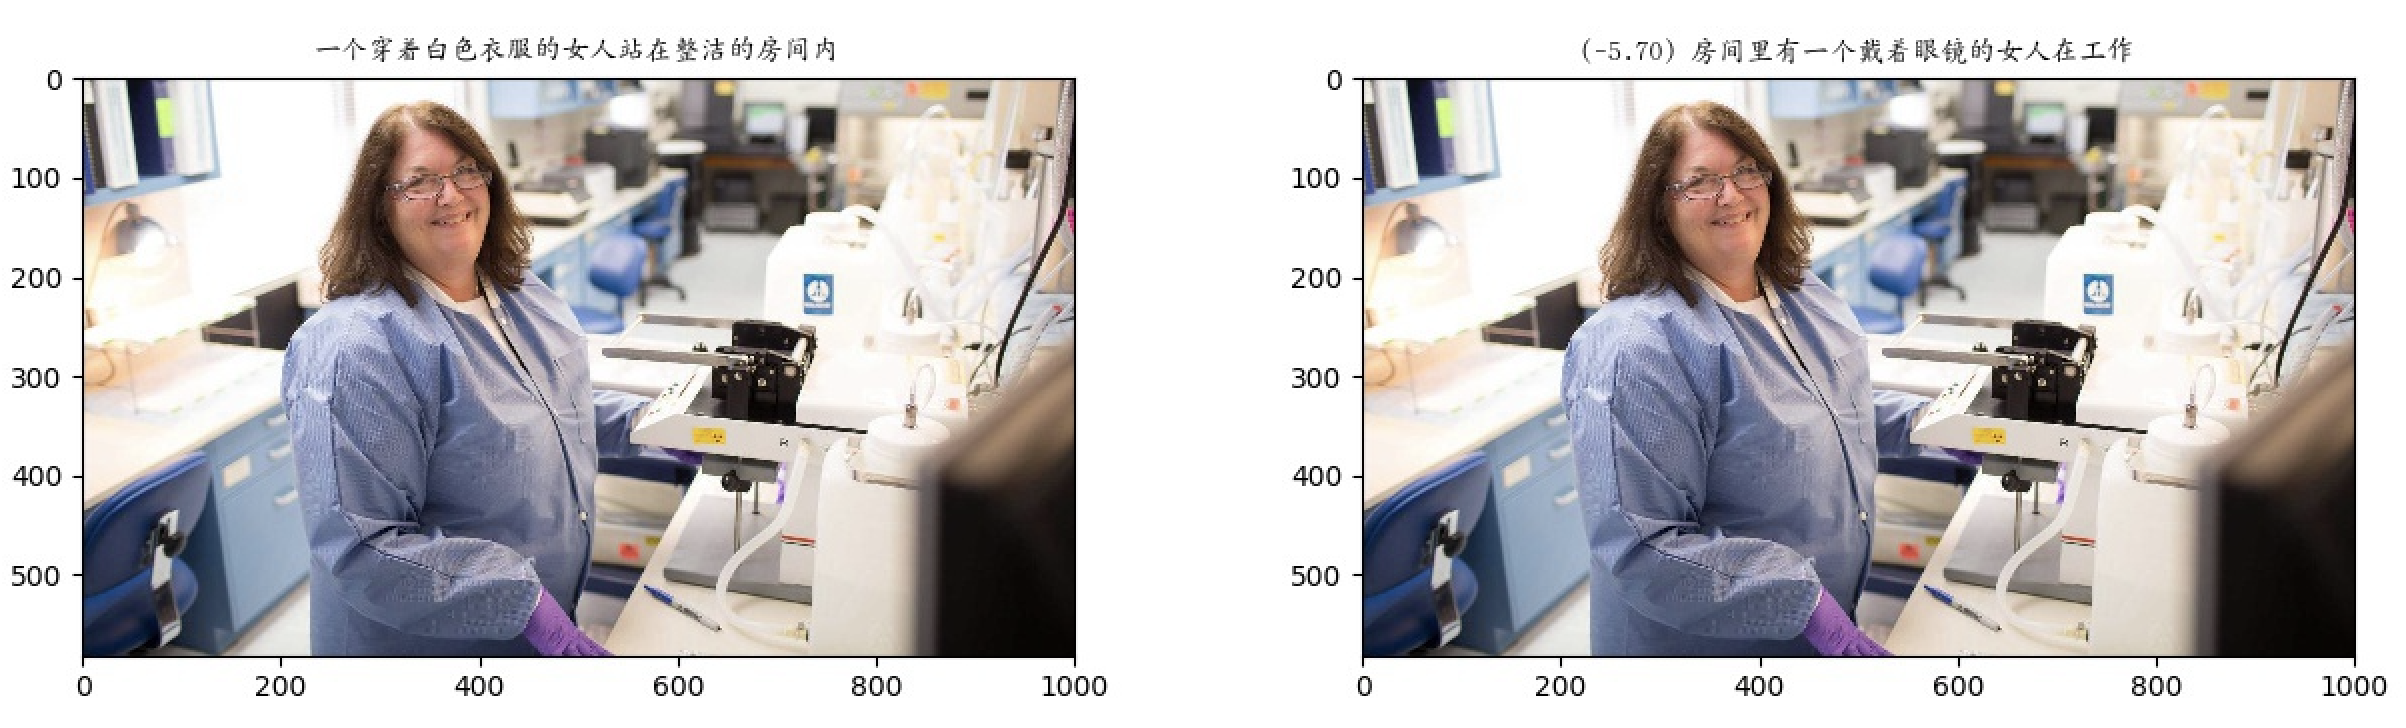
\includegraphics[width=\linewidth]{figures/comparison-3}
	\end{figure}
	
\end{document}